\section{Transformer}

LLMs are primarily based on the Transformer architecture, which has become the foundation for various state-of-the-art NLP models. In this section, we will discuss the main components of the Transformer architecture.

\subsection{Transformer Architecture}

The transformer architecture is a groundbreaking neural network architecture designed for NLP tasks. It was introduced by Vaswani et al. in the paper "Attention is All You Need"\cite{vaswani2023attention} The architecture relies on the self-attention mechanism to process and generate sequences, making it highly efficient and scalable compared to traditional RNNs and LSTM models. The problem in RNNs and LSTMs is that their network sequence makes it hard to process long sentences and, the ability to perform tasks in parallel is affected by sequential computation. Transformer approaches these problems by using encoders, decoders, and self-attention.

\noindent The transformer model is shown in Figure \ref{fig:transformer} below.

\begin{figure}[H]
    \centering
    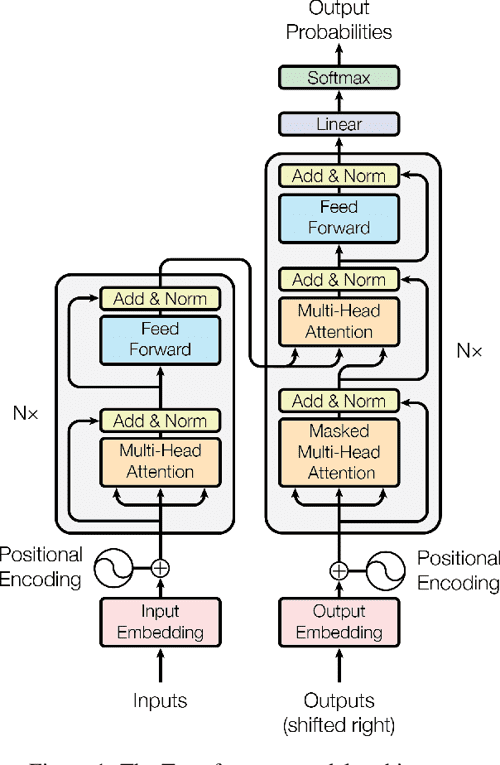
\includegraphics[width=\textwidth,height=6cm,keepaspectratio=true]{transformer.png}
    \caption{
        \it{Transformer architecture model \cite{vaswani2023attention}.}
    }
    \label{fig:transformer}
\end{figure}

\subsection{Components of the Transformer Architecture}

Figure \ref{fig:transformer} depicts the sequence flow beginning at the base of the embedding block, where input and output tokens undergo conversion into fixed-size vectors represented by numerical values corresponding to the tokens. Subsequently, positional encoding is applied to the tokens, assigning them position-specific values to track their sequential order. This step compensates for the absence of recursion and convolution within the network \cite{vaswani2023attention}. Progressing along the input pathway, the encoder stack follows, comprised of \(N\) identical layer structures, each containing two sub-layers: a multi-head attention network and a feedforward network. The output from the encoder is then forwarded to the subsequent encoder. On the output side of the sequence, a decoder stack is present, also composed of \(N\) layers. Each decoder layer features a masked multi-head attention network for outputs, followed by multi-head attention incorporating encoder stack outputs. Analogous to the encoder, a feedforward network concludes the decoder. Normalization is performed between all sub-layers. Subsequently, the decoder output is linearized, and the softmax activation function is applied to transform output token values into a probability distribution. The resulting sequence yields a list of token probabilities, representing the transformer's predictions for suitable tokens given the input sequence.

\subsection{Self-Attention Mechanism}

In the article "Attention is all you need" the self-attention network is called Multi-Head Attention and consists of linearly projecting inputs, Scaled Dot-Product Attention layers,
output concatenation, and finally, projecting the output values \cite{vaswani2023attention}. The self-attention network is introduced in Figure \ref{fig:multi} below.

\begin{figure}[H]
    \centering
    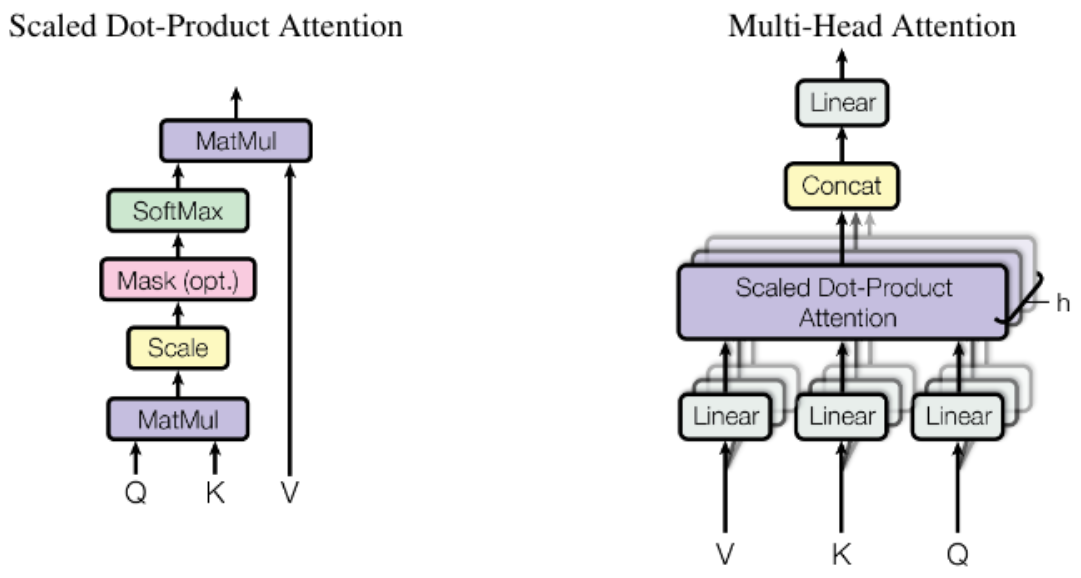
\includegraphics[width=\textwidth,height=6cm,keepaspectratio=true]{multi.png}
    \caption{
        \it{Multi-Head attention network \cite{vaswani2023attention}.}
    }
    \label{fig:multi}
\end{figure}

The network's inputs comprise matrices containing query, key, and value vectors for each token. The matrix \(Q\) represents query vectors, \(K\) corresponds to keys, and \(V\) represents values. To simplify these terms, envision the query as akin to a search engine query initiated by a user, where the key value signifies the title of the search results, and the value encapsulates the content within the titles. These matrices correspond to sentences composed of tokens. Utilizing the scaled dot-product attention mechanism, the network produces tokens with associated attention scores. Multiple self-attention layers, denoted by \(h\), operate concurrently, a process referred to as multi-head attention. This mechanism enables the model to track token positions effectively. The attention scores generated by self-attention can be expressed using Equation \ref{eq:attention}.

\begin{equation}\label{eq:attention}
    Attention(Q,K,V) = softmax(\frac{QK^T}{\sqrt[2]{d_k}})V
\end{equation}

The dot product, performed on matrices \(Q\) and \(K\), is divided by the square root of \(d_k\), representing the dimensionality of the key vectors \cite{vaswani2023attention}. This division serves as a scaling factor. Subsequently, the \(softmax\) activation function is applied to this result, which is then multiplied by \(V\) to obtain the attention matrix. This process is repeated \(h\) times to generate multiple multi-head attention matrices. These matrices are subsequently concatenated into a single linearized matrix, which is then fed into the feedforward network.

The feedforward network employed within the transformer architecture shares similarities with the network outlined in Figure \ref{fig:transformer}, but with variations in the number of layers, input and output dimensions, activation function, and other parameters across different models. In the "Attention is all you need" article, two linear transformations with ReLU activation were utilized, featuring output and input dimensions of \(d_{model} = 512\), and an inner-layer dimensionality of 2048 \cite{vaswani2023attention}. Within the realm of LLMs, some of these parameters can be regarded as hyperparameters, exhibiting variability across models. For instance, in the Chinchilla  model, the dimensionality is \(d_{model} = 8192\), with the feedforward network size consistently four times the former value \cite{hoffmann2022training}.

\subsection{Variants of Transformer Architecture}

Various LLMs are built on top of the Transformer architecture with slight modifications or adaptations. Some popular variants include:

\textbf{GPT:} The Generative Pre-trained Transformer (GPT) is an autoregressive model that utilizes only the decoder part of the Transformer architecture to generate text \cite{openai:gpt}.

\textbf{BERT:} Bidirectional Encoder Representations from Transformers (BERT) is based on the encoder part of the Transformer architecture and is pre-trained using masked language modeling and next sentence prediction tasks \cite{devlin2019bert}.

\textbf{T5:} The Text-to-Text Transfer Transformer (T5) adapts the original Transformer architecture to a unified text-to-text format, enabling it to be used for various NLP tasks with minimal task-specific modifications \cite{raffel2023exploring}.